\section{Search strategy}
\label{sec:strategy}

The present section provides a brief overview of the dominant backgrounds, how they are suppressed,
and how the remaining background is estimated.

There are three types of backgrounds:
\begin{itemize}
\item Single lepton background
\item Lost lepton background
\item Background from $Z\to\nu\nu$
\end{itemize}

\subsection{Single Lepton background}

%This is the largest background for any search in the single isolated lepton plus jets plus \MET final state.
%It can be reduced dramatically with a combination of transverse mass and missing transverse momentum.
%
For any search in the single isolated lepton plus jets plus \MET final state, this background is the largest before any signal selection is applied. However, it can be reduced dramatically with a combination of transverse mass (\MT) and \MET.

Figure~\ref{fig:strategy:recoMT:W} shows the shape of the transverse mass distribution overlaid for \MET $\ge$ 50, 150, and 250\GeV
for W+jets Monte Carlo. It clearly shows the kinematic edge due to the W mass, and how this edge becomes more and more
dramatic as \MET is increased.

\begin{figure}
\subfigure[Reconstructed \MT distribution in reconstructed \PW($\ell\nu$)+jets events. The \PW~boson mass edge becomes steeper with increasing \MET requirement.]{
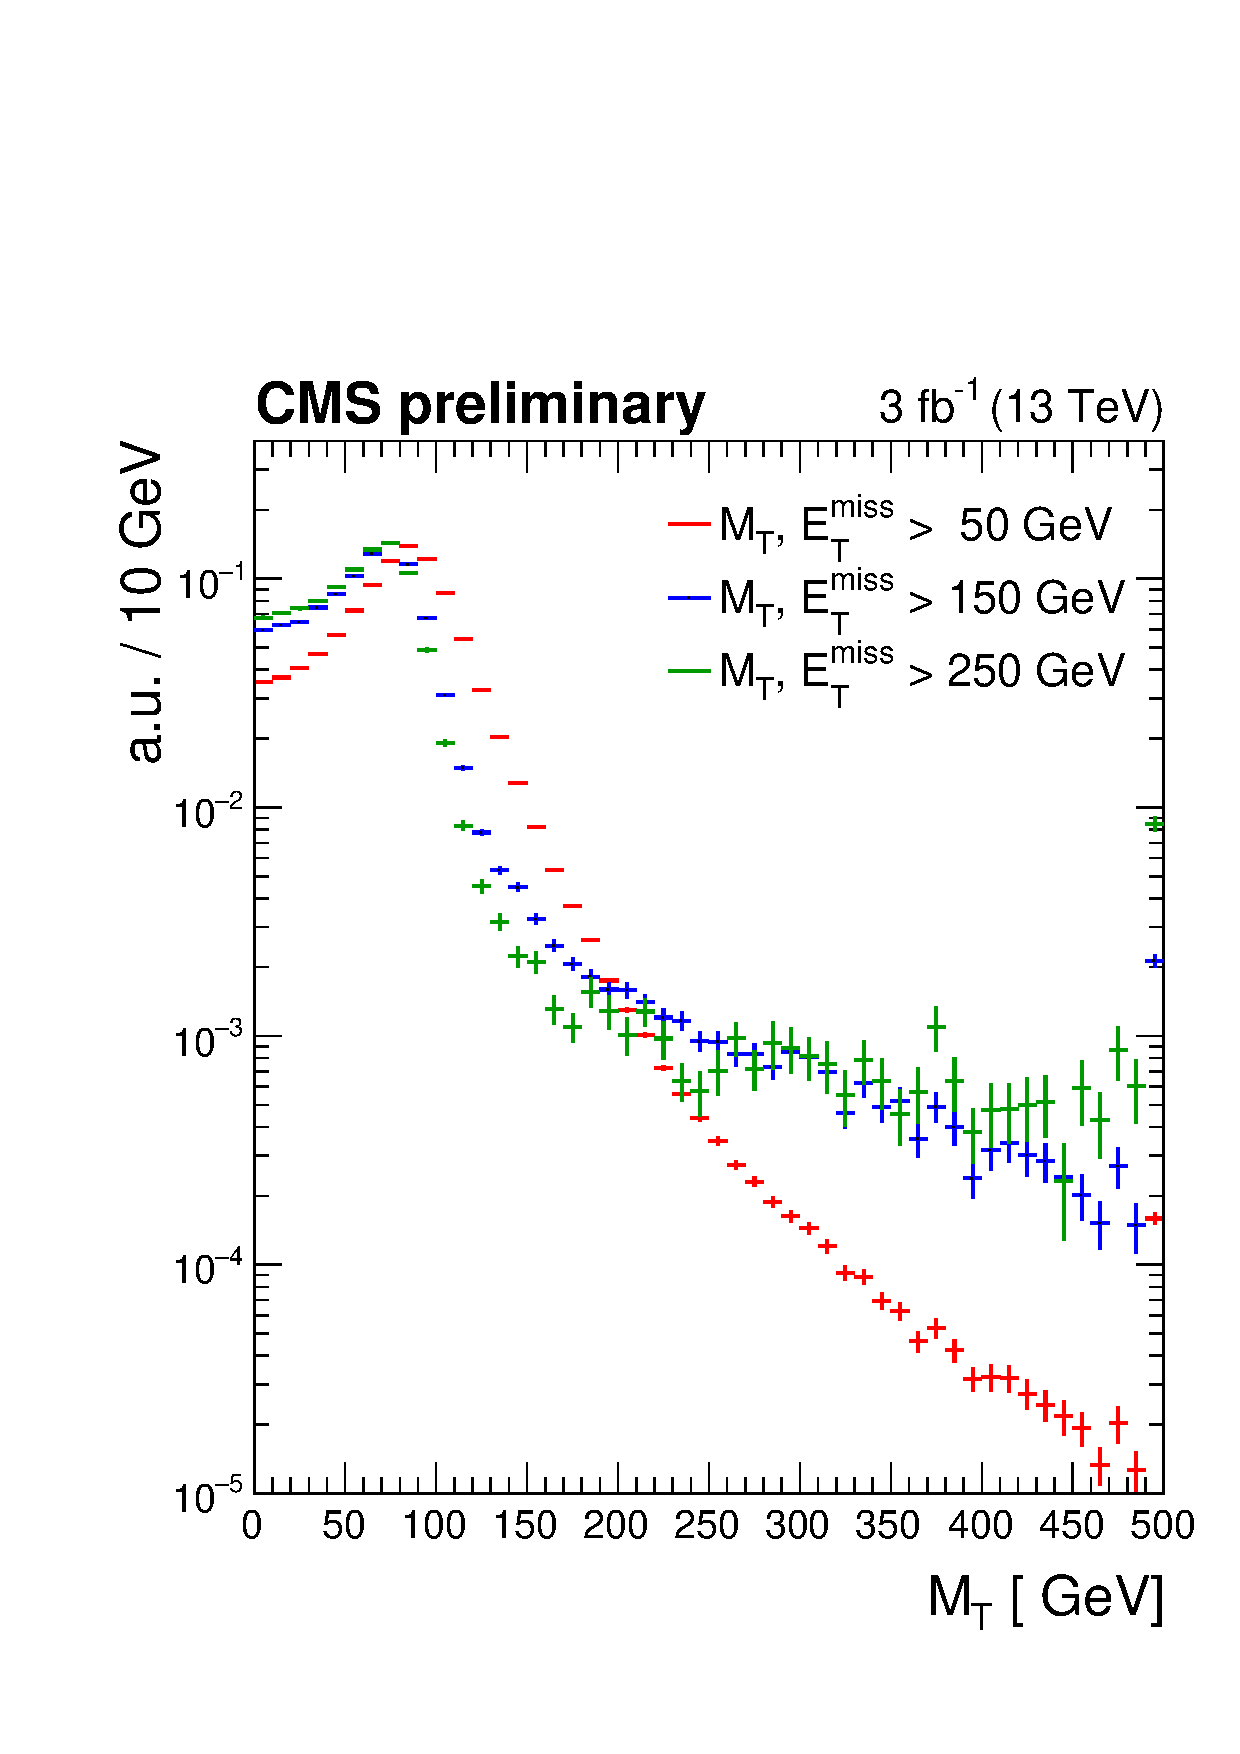
\includegraphics[width=0.3\textwidth]{Figures/Strat_MT_W.pdf}
\label{fig:strategy:recoMT:W}
}
\hspace{5pt}
\subfigure[Reconstructed and generator-truth \MT distribution in \PW($\ell\nu$)+jets and $\cPqt\cPaqt(\to1\ell)$+jets events.]{
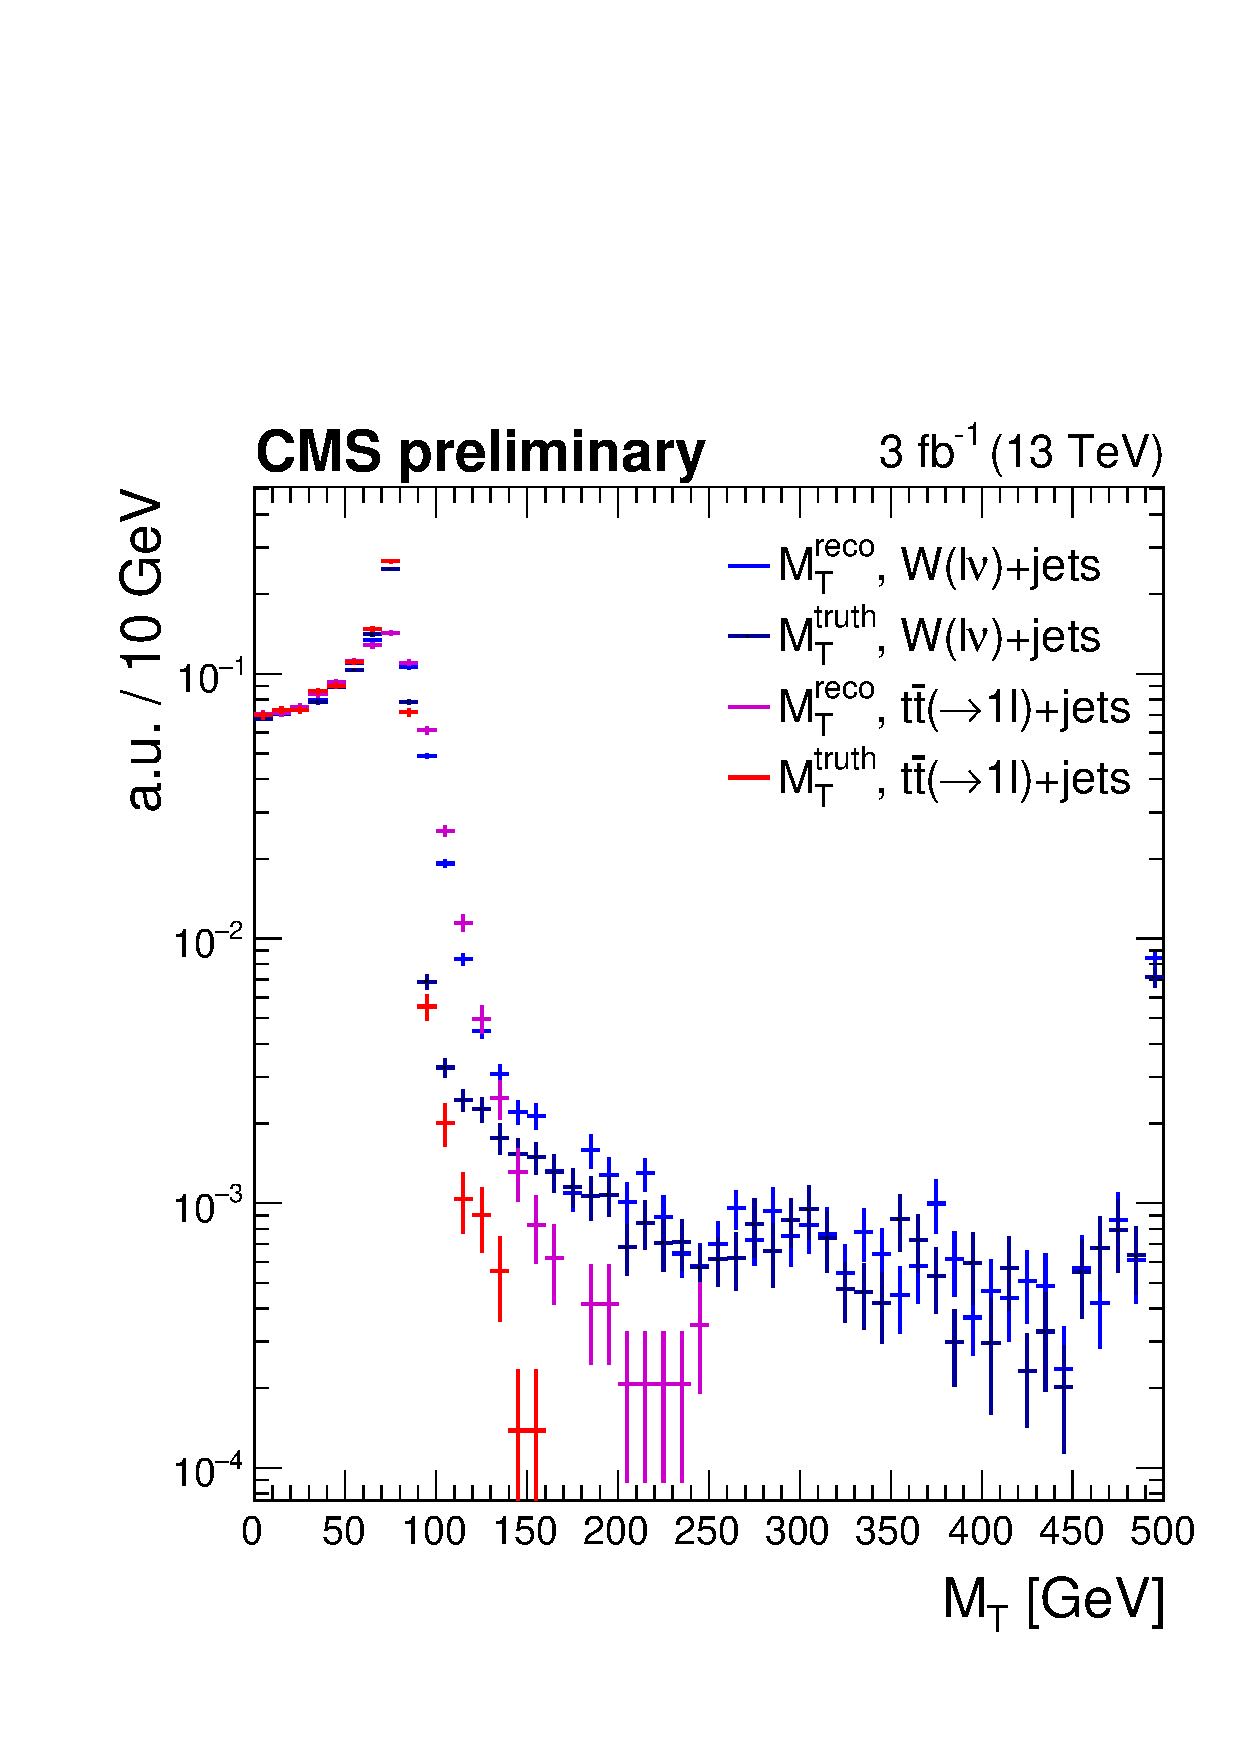
\includegraphics[width=0.3\textwidth]{Figures/Strat_MT_WTop.pdf}
\label{fig:strategy:recogenMT:Wttbar}
}
\hspace{5pt}
\subfigure[Generator-truth \MT distribution in reconstructed \PW($\ell\nu$)+jets events. The \PW~boson mass edge becomes steeper with increasing \MET requirement.]{
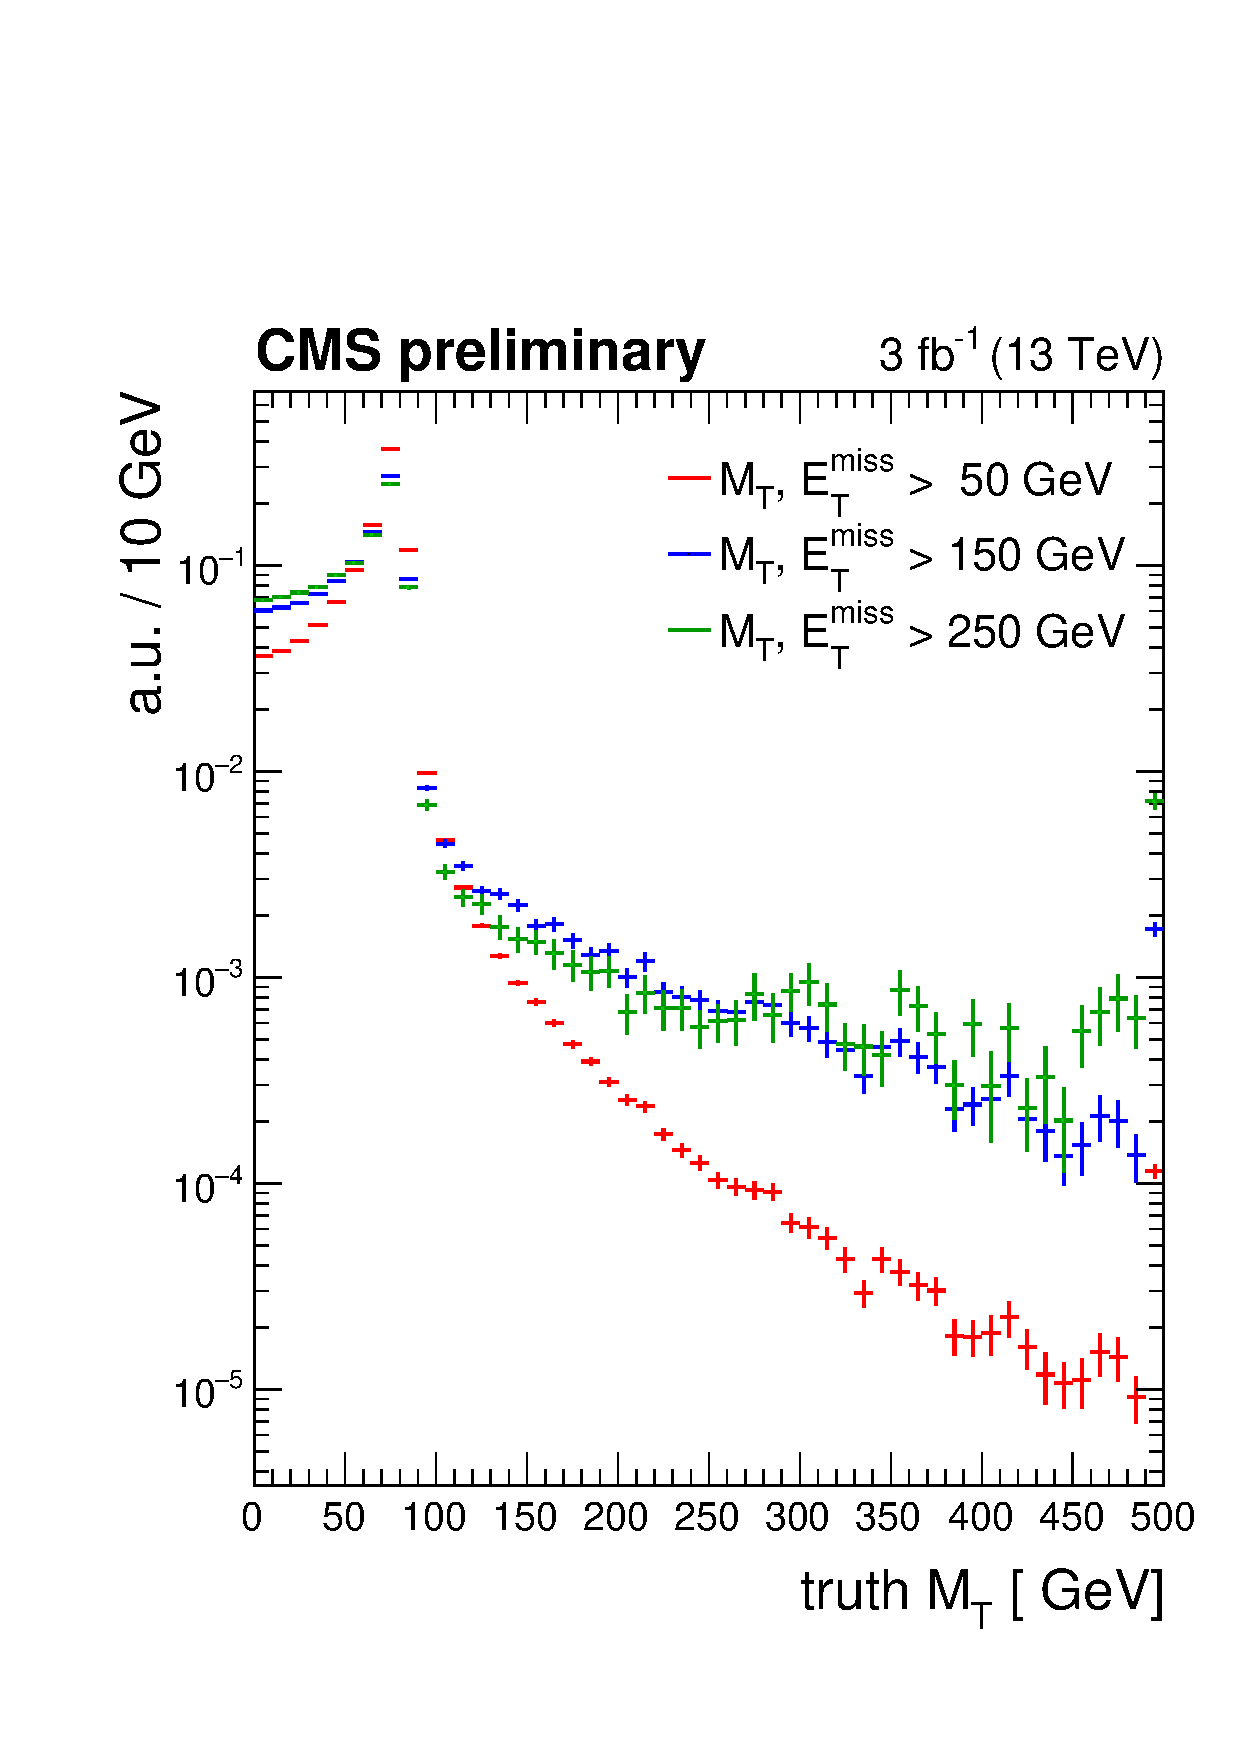
\includegraphics[width=0.3\textwidth]{Figures/Strat_MTtruth_W.pdf}
\label{fig:strategy:truthMT:W}
}
\caption{\label{fig:strategy:MT} \MT distributions.}
\end{figure}

Figure~\ref{fig:strategy:recogenMT:Wttbar} shows the shape of the transverse mass distribution for \MET $\ge$ 250\GeV, at least 2 jets and only one lepton 
at generator level, all with \pt $\ge$ 30\GeV. The Figure overlays generator and reco level transverse mass for W+jets and ttbar.
In both cases, we plot as generator level the transverse mass of the lepton neutrino pair. 
We see from this figure that the high transverse mass tail at generator level have dramatically different shapes for W+jets and ttbar. 
This is due to the fact that the top mass functions as a kinematic constraint on the W mass in ttbar, but no such constraint exists in W+jets.
As a result, the high transverse mass tail in ttbar 1-lepton events is dominated by \MET resolution effects, while for W+jets it is
largely driven by physics, i.e. the width of the W.

From these two simple figures, we learn that fundamentally, the 1-lepton background after \MT and \MET cuts is a complicated 
mix of relative production cross section of W+jets and ttbar, as well as \MET resolution effects. 
In practice, we picked our baseline cuts \MET$\ge$250\GeV and \MT$\ge$ 150\GeV such that 
the Monte Carlo predicts the 1-lepton ttbar background to be negligible in all our signal regions compared to W+jets.
This simplifies the analysis dramatically, and makes us only mildly dependent on systematic errors in the \MET resolution and/or
relative cross sections of ttbar and W+jets.

We then use zero b-tag control regions to normalize the W jets background in data. 
The details of these regions is a trade-off between statistics and ``extrapolation lever arm''.
A larger lever arm means better statistics in the control region but larger systematics due to the larger extrapolation.
For this analysis, we chose to extrapolate only in two variables, b-tagging and \MET for the W jets background.

In addition, we show via a combination of data and MC that 1-lepton ttbar background is indeed negligible, as expected,
and can thus be taken from Monte Carlo.

\subsection{Lost Lepton background}

The dominate background after \MET and \MT cuts as described above is ttbar with both W's decaying leptonically.
This background dominates even after carefully optimized 2nd lepton veto. We refer to this as "lost lepton" background
because typically the second lepton is either a hadronic tau that is not reconstructed, or an e,$\mu$ that is not isolated, or outside
\pt or $\eta$ acceptance of our lepton veto.

We estimate this background from dilepton control regions in data times transfer factors from Monte Carlo, and scale factors to account
for known differences in lepton efficiencies between data and Monte Carlo. 
The details are more complicated as this simplistic overview because we need to account for potential differences in 
gluon or quark radiation between data and Monte Carlo that affects lost hadronic tau and lost e or $\mu$ differently.

\subsection{Background from \texorpdfstring{$Z\to\nu\nu$}{Znunu}}

The dominant source of $Z\to\nu\nu$ in any of our signal regions is from ttbar + Z production where one of the two W's from top decay
decays leptonically. This background is not accounted for in either of the two previous estimation strategies in any way.
At some point in 2016, when we have plenty of data to measure both ttZ and tt$\gamma$ with $Z\to \ell\ell$ we might be able to define
a dedicated control region for ttZ. However, for the 2015 dataset, we will simply estimate ttZ from Monte Carlo, and use renormalization 
and factorization scale uncertainties evaluated as suggested by the CMS generator group as systematic uncertainty on this background.




